\section{Event Isolation Flagging}
	
	One challenge of increasing the readout speed of the detector is processing the data that is produced.
	Because of this, any pre-processor functions executed in the FPGA reduces the load and processing time of the computer system.
	One area where the DAQ's FPGA will be used for this purpose is in \underline{E}vent \underline{I}solation \underline{F}lagging (EIF).
	\par
	When particles traverse the VELO there is a finite probability that they will pass though the boundary of two or more Super Pixels.
	This will cause multiple SPPs to be created for the same particle path.
	For such paths, the computer is required to search all SPP corresponding to the event, and identify SPP's that relate the the same particle track. However, as the computer doesn't have information on which SPP's do and do not have adjacent SPP's, the computer is required to search for neighboring SPP's for each SPP in the BCID. This is an inefficiency which can be solved withing the FPGA, before the computer processes the data.
	\par
	The aim of EIF is to identify the SPPs that completely describe the particles interaction with the module and flag such SPP's as isolated.
	The computer can then save time by negating the need to search for adjacent SPP's.
	By speeding up to the processing of such tracks, the pile-up of data is reduced.
	This thus reduces the probability of the computer needing to reject incoming data or for the detector to stop collecting data.

	\subsection{Router and MEP Interface} % (fold)
	\label{sub:router_and_mep_interface}

		Retrieving and delivering BCID information withing the FPGA is a challenge in its self.
		In the router data is not processed in BCID order, instead information from many BCID's are processed simultaneously.
		Adding complication, the EIF-MEP interface must identically match that of the Router-IEF.
		This is because the IEF module is not a priority for implementation in the final production for the DAQ FPGA.
		Thus, the IEF module must be easily removable without the need for a significant re-design.

		The decision was made to implement swinging buffers between the Router-EIF and EIF-MEP interfaces.
		Each swinging buffer consists of two sets of 16 RAMs, each containing the SPPs of 32 BCIDs and an additional count ram, that contains the number of SPPs in each BCID.
		During one swing cycle, one of the interfacing modules can write information to one set of RAMs in the buffer while the second module reads from the second set of Rams.
		This approach has two main benefits: firstly there can be no read-write conflicts where the EIF or MEP read data from a BCID before writing is complete; secondly the calculation deciding if a BCID can be processed before being overwritten is significantly simplified.
		In addition, the swinging buffer allows for the parallelization of EIF modules.
		This reduces the load on each EIF unit and prevents the BCIDs from being bypassed due to lack of processing time.

		\subsubsection{RAM Interfacing} % (fold)
		\label{sub:ram_interfacing}
			

			Communicating with a RAM block, either to read (rd) or write (wr), requires the use of three signals.

			\begin{description}
				\item [Enable (en)] signaling to the RAM to read or write.
				\item [Address (addr)] identifying the address in the RAM to read or write from.
				\item [Data] This signal is used to transfer the data into out of the RAM.
			\end{description}

			On the falling edge of the clock (clk), if the wr\textunderscore en or rd\textunderscore en signals are high, the RAM will write the wr\textunderscore data signal to the specified address or output the data stored in the address to the rd\textunderscore data signal respectively. 
			The count RAM (ct) is the only exception as it does not have a read enable.
			Instead the count RAM will update the data signal every falling edge to whatever address the ct\textunderscore addr signal specifies.

			The RAMs used in the FPGA do not have a large enough output bandwidth to output the whole of a BCID in one address.
			Each address in the RAM contains the information of 16 SPPs.
			Therefore, if a BCID contains greater than 16 SPPs its required to iterate over several addresses on the RAM and combine the data to form a complete set of SPPs.
			Similarly, when writing more than 16 SPPs one must write the data incrementally to adjacent addresses.
			One consequence of this is that the RAMS must be flashed clear on the buffer swing to prevent old data being used twice.

			In addition to the 16 SPP max read/write speed, each BCID has only 32 address.
			Therefore a max of 512 SPPs can be stored in one BCID.

			\begin{figure}[ht]
				\centering
				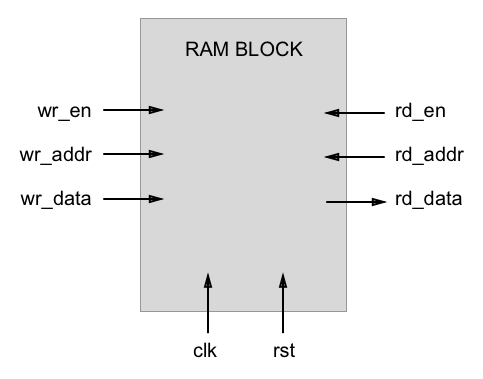
\includegraphics[width=0.7\textwidth]{RAM_BLOCK}
				\caption{A diagram showing the signals required for a simple RAM block.}
				\label{fig:ram_diagram}
			\end{figure}
		% subsection ram_interfacing (end)
	
	% subsection router_and_mep_interface (end)

	\subsection{Top Level EIF Module} % (fold)
	\label{sub:top_level_processing}
	
		The EIF data processing comprises of two main steps.

		\begin{itemize}
			\item Bubble sort the SPP's by row ID.
			\item Compare SPP row ID to adjacent SPP's and compute if isolated. 
		\end{itemize}

		One of the major constraints of the data processing is the max number of SPP's that the Bubble sort can accept.
		It is therefore necessary to include in a bypass system to the process that allows BCID's with too many SPP's to be passed onto the next stage without being processed.
		Such BCID's will be processed in the same way for the rest of the FPGA and CPU processes, but will not benefit from the time saving property of the EIF.

		As such the top level entity contains three child entities.

		\begin{description}
			\item[Active Controller] \hfill \\
				This entity reads in the BCID's to an array of data processors and writes the results to the output ram.
			\item[Interface FIFO] \hfill \\
				This \underline{F}irst \underline{I}n \underline{F}irst \underline{O}ut entity is written to by the Active Controller and is used to inform the Bypass Controller of which BCID's have and have not been bypassed.
			\item[Bypass Controller] \hfill \\
				This entity passing data across the EIF system without data processing.
		\end{description}

		\begin{figure}[ht]
			\centering
			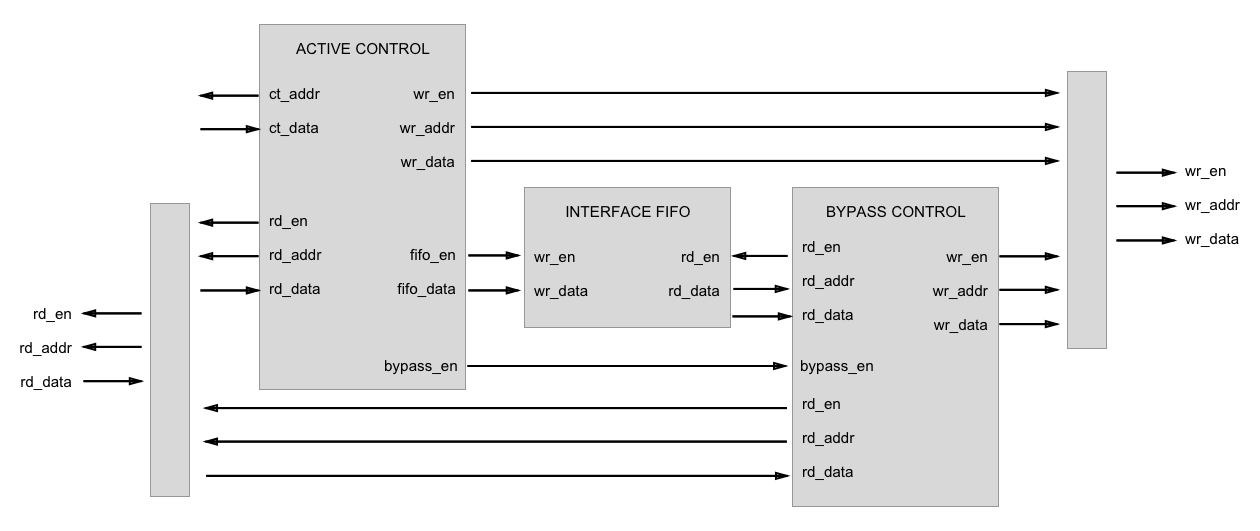
\includegraphics[width=\textwidth]{EIF_BLOCK}
			\caption{A diagram showing the signal arrangement of the top level EIF entity.}
			\label{fig:EIF_BLOCK}
		\end{figure}

		By monitoring the bypass\textunderscore en signal, the EIF top level diagram can detect whether the Active Controller or Bypass Controller read and write signals need to be routed to the outputs.
		This can be seen in Figure~\ref{fig:EIF_BLOCK} as the two slim grey rectangles at either side of the diagram.
		When the bypass\textunderscore en signal is low, the Active Controller is linked with the RAMs.
		The signals pass though the EIF top level entity without delay.
		Conversely, when the bypass\textunderscore en signal is high, the Bypass Controller signals pass the the RAMs.

		\subsection{Active Controller} % (fold)
		\label{sub:active_controller}

		\begin{figure}[ht]
			\centering
			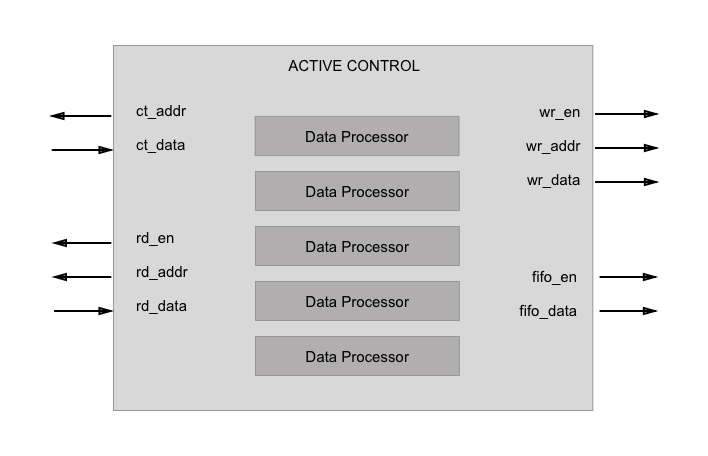
\includegraphics[width=0.8\textwidth]{ACTIVE_CONTROL}
			\caption{A diagram showing the structure of the Active Controller entity. This diagram shows the presence of five Data Processor entities, however any number of Data Processors may be used.}
			\label{fig:active_control_diagram}
		\end{figure}
		
		At the beginning of a swinging buffer cycle, the active control checks if the first BCID both has data and can fit into the data processing units.
		Then, if the BCID is suitable for processing it is read into a data processor and a value of 0 is written to the Interface FIFO and the Active Controller moves to the next address.
		If the number of SPPs is too large or if it is zero, the number of SPPs is written to the Interface FIFO, and again the Active Controller movies to the next address.

		Once the Active Controller has finished with the final address and all data processors have had their output written to the MEP Interface RAMs, the bypass\textunderscore en signal is set high and the Active Controller waits until the next swinging buffer.
		
		% subsection active_controller (end)

		\subsection{Data Processor} % (fold)
		\label{sub:data_processor}

			\begin{figure}[ht]
				\centering
				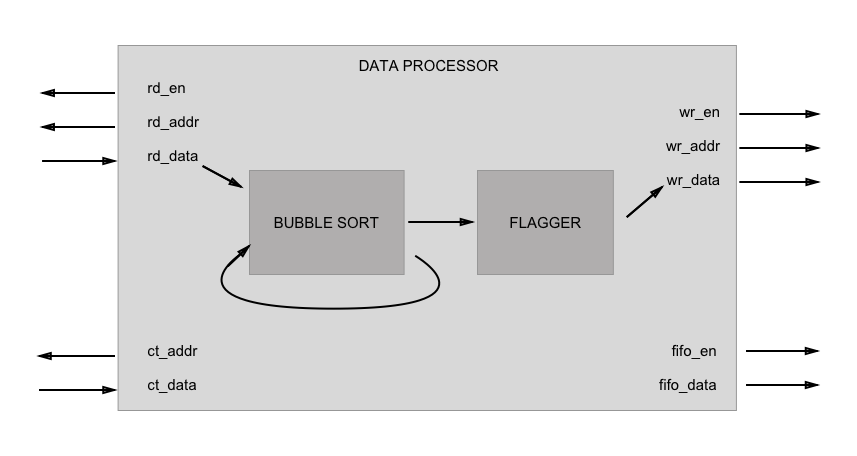
\includegraphics[width=0.8\textwidth]{DATA_PROCESSOR}
				\caption{A diagram showing the structure of the Data Processor entity. }
				\label{fig:data_processor_diagram}
			\end{figure}

			The data processor computes the sort algorithm, passes the sorted data to the flagging module and then outputs the data.
			Not shown in Figure~\ref{fig:data_processor_diagram} for simplicity, the data processor uses validation signals to communicate with the active controller to ensure it is not passed data too early and that the data is outputted correctly after the process.

			In addition to the SPPs being passed into the Data Processor, the BCID and number of SPPs must also be given.
			The BCID is used later when writing the information to the MEP Interface RAM and the SPP count is used in the bubble sort process.

		\subsubsection{Bubble Sorting}

			Bubble sorting is the process of sequentially comparing adjacent elements of a list and swapping the element if necessary.
			For example, if sorting into ascending order and comparing the value 5 and 3, a swap would be needed.
			However, comparing 3 and 5 in the same example would not need a swap.
			When sorting an arbitrary list, we can define an `even-odd' comparison as one comparing an even placed element with an odd one (i.e. element 4 with element 5).
			An `odd-even' comparison is the logic opposite (i.e. element 5 with element 6).
			\par
			Bubble sorting, when implemented in series processing, is a relatively slow sorting algorithm.
			At worst case, Bubble sorting requires $n^2$ iterations to complete the sort of a list of size $n$.
			However, FPGAs can easily parallel process.
			By making $\frac{n}{2}$ comparisons simultaneously (all even-odd or odd-even pairs), FPGA Bubble Sorting in the worst case scenario only requires $n$ iterations. This is made clear in Figure~\ref{fig:sorting}.

			\begin{figure}[ht]
				\centering
				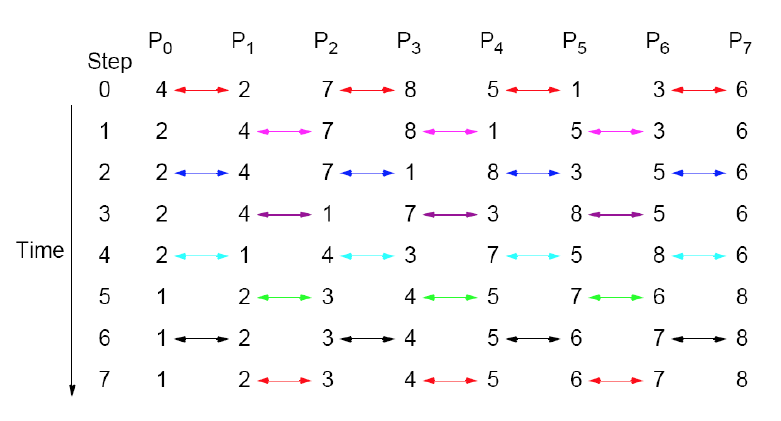
\includegraphics[width=0.7\textwidth]{sorting_diagram}
				\caption{A diagram showing Bubble Sorting in an FPGA.}
				\label{fig:sorting}
			\end{figure}

			When bubble sorting in the data processor, the SPPs are cycled around a feedback loop until sorted.
			There are three approaches to calculating when the sort is complete:

			\begin{description}
				\item [Static:] \hfill \\ Sorting for the worst case scenario assuming the max number of SPPs have been inputted.
				\item [Semi-Static:] \hfill \\ Sorting for the worst case scenario for the actual number of SPPs inputted.
				\item [Dynamic:] \hfill \\ Checking if swaps have been made after each iteration and classing the data as sorted once the odd and even comparisons sequentially make no swaps.
			\end{description}			

			Intuitively, the semi-static method is superior to the static method, thus the static option is immediately rejected.
			There are pros and cons of the both the semi-static and dynamic options. 
			The dynamic sort will save time on almost sorted data sets, however for short or heavily disordered datasets the dynamic sort isn't every efficient as it requires two cycles without comparison to exit.
			The semi-static method, while waisting time on almost sorted data, uses less resources than the dynamic method and for smalled data sets there is less opportunity to save time.

			Deciding between the semi-static and dynamic sorting methods required further research.
			The two methods where simulated and compared on time saved by implementing a dynamic sort over semi-static.
			The data used was a time ordered simulated output of the VELO.
			If the dynamic sort took longer than the semi-static, it was given a time saved of zero, this is because the dynamic sort can be setup with a semi-static exit strategy.

			\begin{figure}[ht]
				\centering
				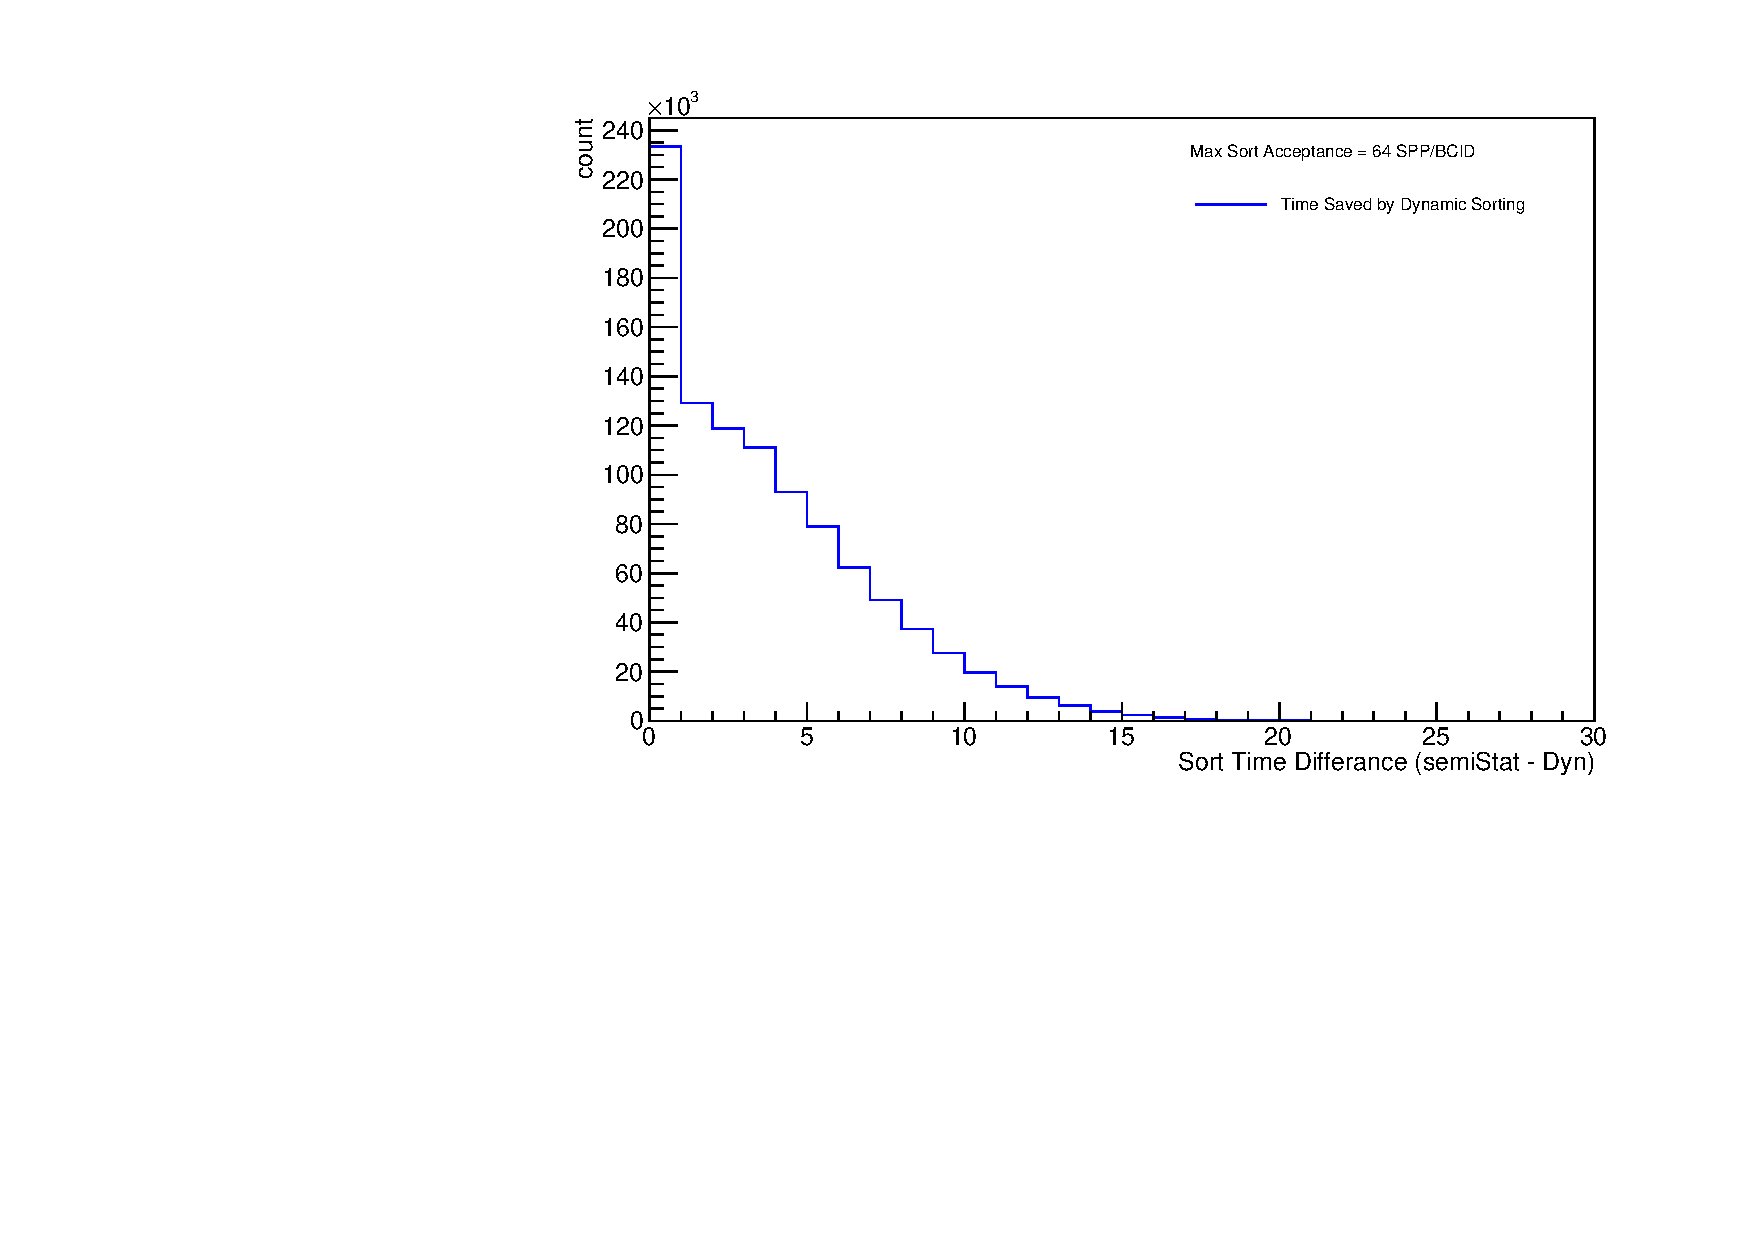
\includegraphics[width=0.49\textwidth]{time_saved_by_dynamic_sort_1d}
				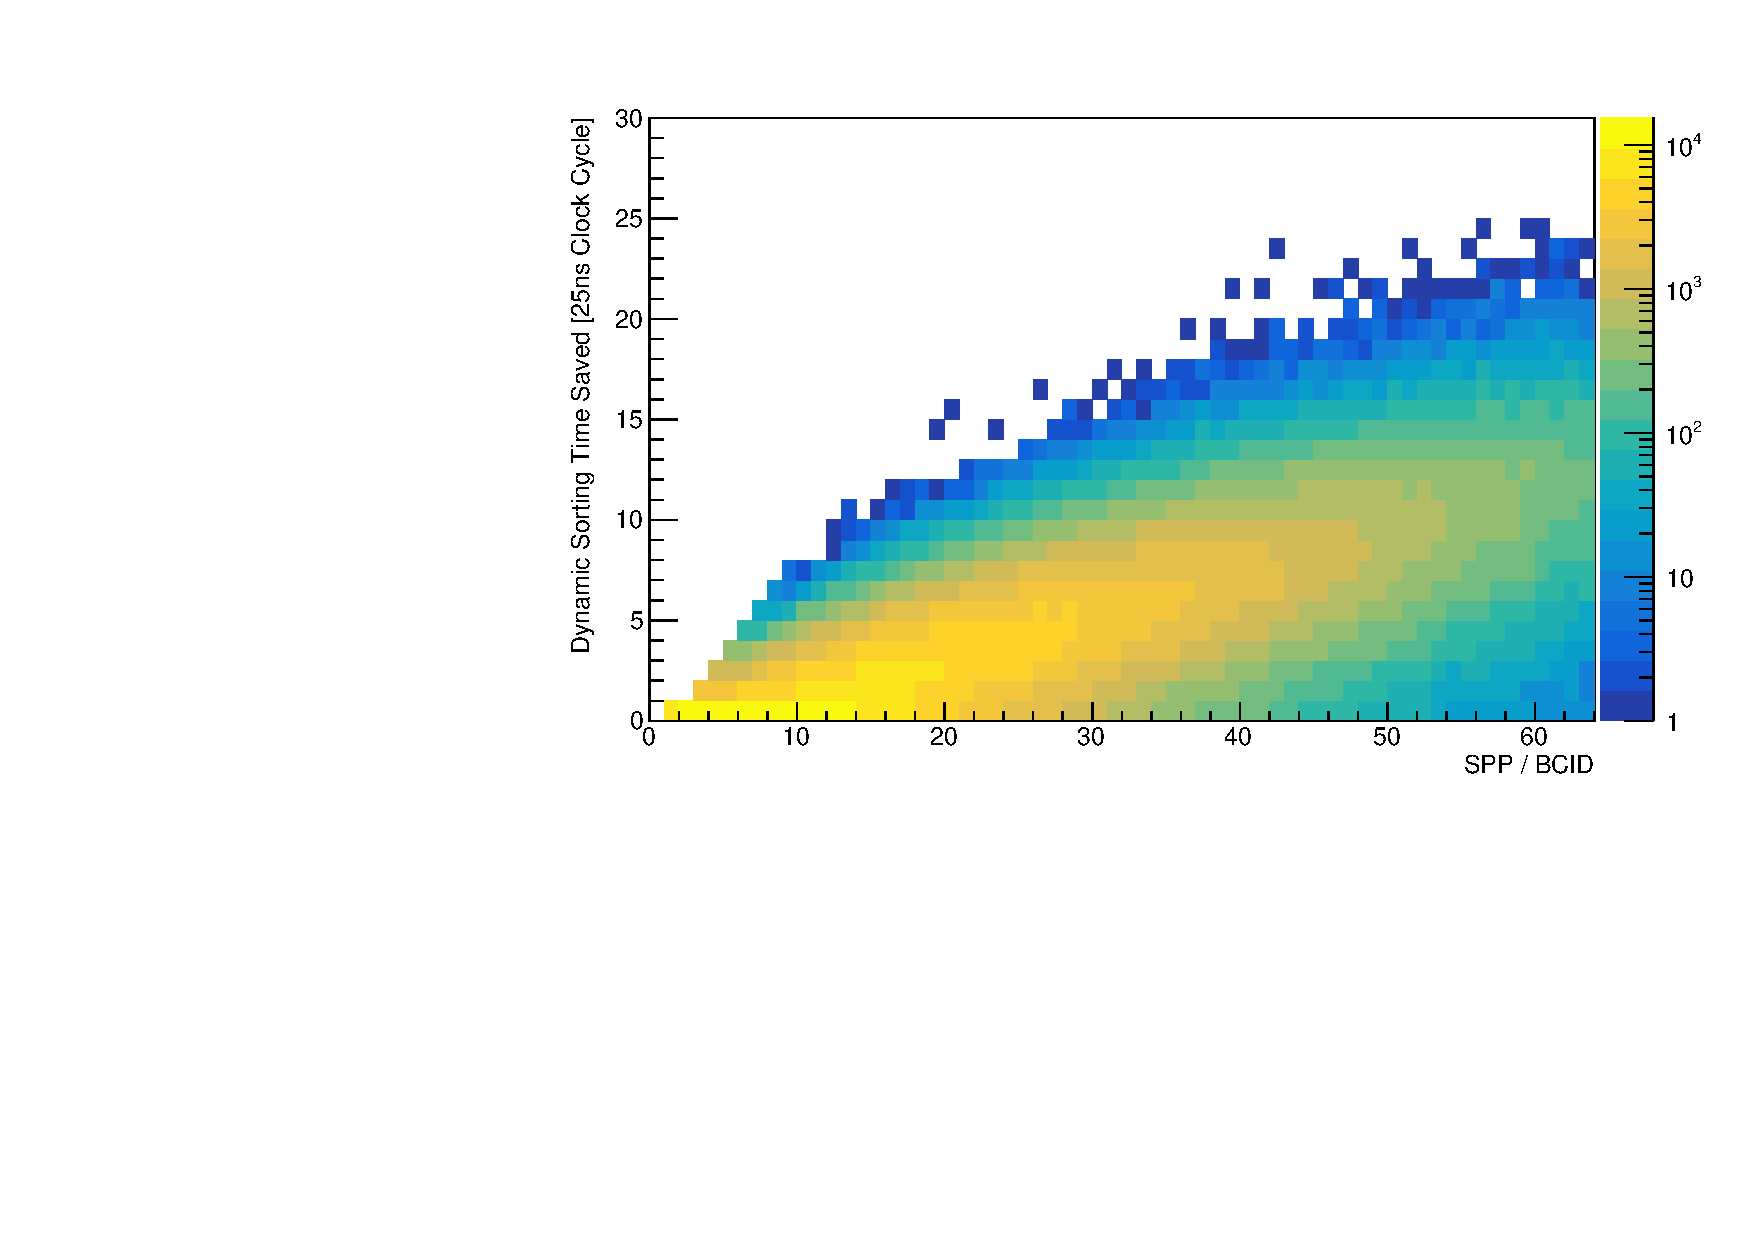
\includegraphics[width=0.49\textwidth]{time_saved_by_dynamic_sort_2d}
				\caption{The time saved by implementing a dynamic sort method over a semi-static method. The left graph show absolute frequency of time saved. The right graph shows how the distribution of time saved relates the number of SPPs, plotted on a log(z) scale.}
				\label{fig:dyn_stat_comp}
			\end{figure}			

			It is clear from Figure~\ref{fig:dyn_stat_comp} that the dynamic sort method does not significantly reduce the sort time.
			For this reason, the decision has been made to implement a semi-static method.
			This will reduce the resources usage of the EIF module, while not significantly increasing the time required to sort the data.

		% subsection data_processor (end)

			\subsubsection{Isolated SPP Tagging} % (fold)
			\label{sub:isolated_spp_tagging}
			
			Inside the Flagger entity shown in Figure~\ref{sub:data_processor}, the flagger compares each SPP in the BCID against the adjacent SPPs.
			If the row ID of both adjacent SPPs is greater than 1 row different, the SPP is classed as isolated.
			This is shown by setting the most significant bit of the SPP to 1.

			In the special case that the SPP is at the edge of the ASIC chip, it is never flagged as isolated.
			This is because other SPPs from adjacent sensors may also relate to the same track.
			However, as the two half modules are processed in different data channels, this deduction cannot me made until the data is combined in the CPU.

			Furthermore, two isolated SPPs that happen by random chance to be in the row but different column is not be flagged.
			With the pixel density of the ASIC chip, this situation is considered too unlikely to warrant further sorting and checking.
			If two isolated SPPs are in the same or adjacent columns, the lack of isolation flag will not affect the CPU processing.
			The SPPs will be checked for neighboring SPPs and when none are found, treated the same as isolated SPPs.
			While this is less time efficient in the CPU the extra processing required to avoid such a situation would negate the benefits.

			\subsubsection{Max SPP Count Per BCID} % (fold)
			\label{sub:max_spp_count_per_bcid}
			
			In order to determine the max number of SPPs the data processor should accept without the need to bypass, the data was analysed to determine the fraction of data that would be accepted at different cutoff values.
			This analysis focuses on two conflicted ideals, the data processor must be able to processor the majority of the data while reducing the amount of resources required.

			\begin{figure}[ht]
				\centering
				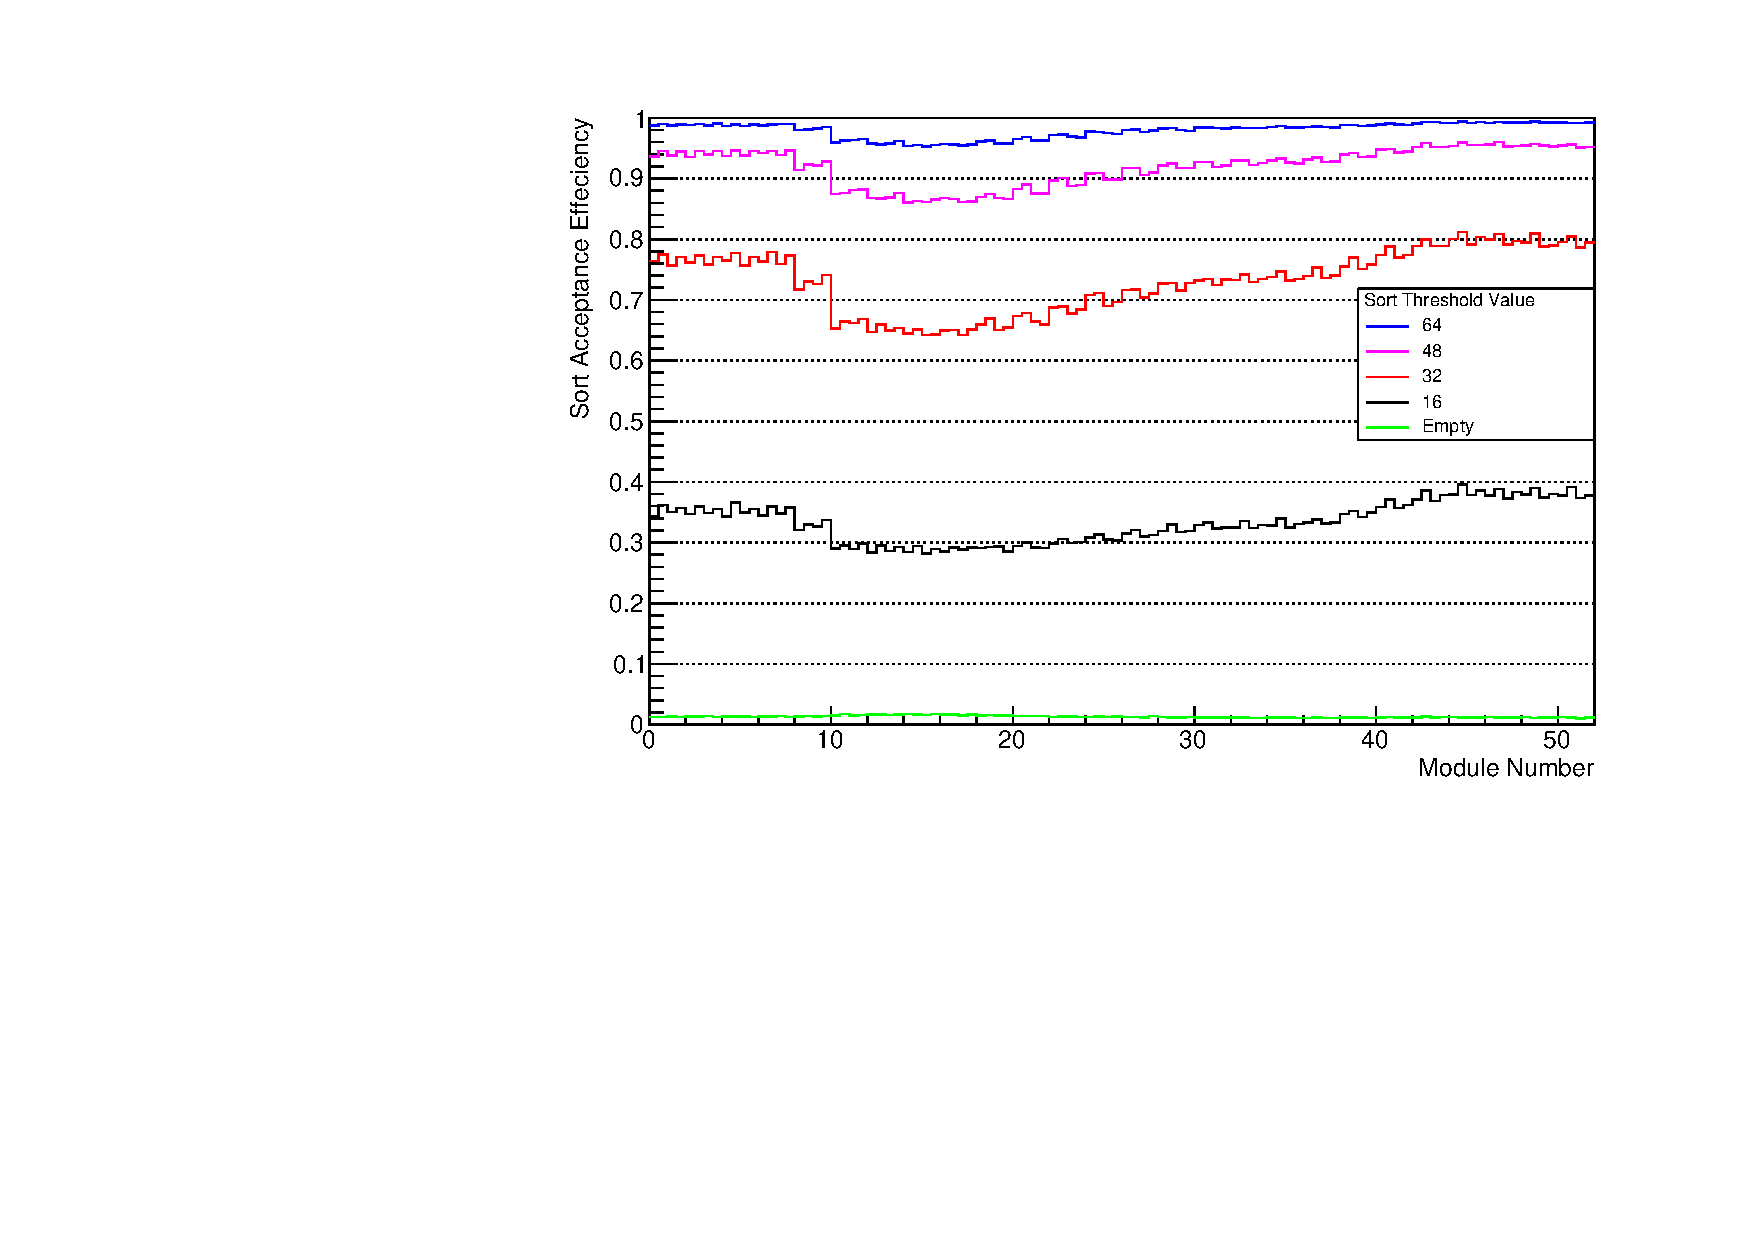
\includegraphics[width=0.8\textwidth]{Sort_Acceptance_Efficiancy}
				\caption{The fraction of BCID's accepted at different threshold values.}
				\label{fig:sort_acceptance}
			\end{figure}

			The data structure in Figure~\ref{fig:sort_acceptance} is as expected.
			The modules around 15 are closest to the interaction point and thus have higher occupancy.
			It is therefore expected that these modules will accept less BCID's for data processing.

			Furthermore, there is a diminishing return on the faction of data accepted.
			A threshold value above 64 would not yield a significant increase in the number of accepted BCID's.
			The value of the sort acceptance, however, is easily modified in the VHDL code and can thus be fine turned once the true resources are calculated.

	\subsection{Bypass Controller} % (fold)
	\label{sub:bypass}
		
		The Bypass controller is the simplest of the entities the EIF.
		Once the bypass\textunderscore en signal is received as high by the Bypass Controller, the information from the Interface FIFO is read in one by one.
		If the value read in is zero, the corresponding BCID does not require bypassing.
		If the value is greater that zero, the corresponding BCID is read out of the Router Interface RAMs and wrote into the same address of the MEP Interface RAMs.
		This continues until the Interface FIFO is empty, at which point the Bypass Controller waits for its enable signal to rise back to high.
		At this point the swinging buffer will have swung, the Active Controller will have finished is process and it will be time for the Bypass Controller to begin its process again.

		For each BCID that is bypassed, the time taken is only two cycles longer than the total time it would take to just read or write the data.
		This is because one clock cycles is used to read in from the FIFO and identify that the BCID requires a bypass, and one clock cycle is used to move the data from the read-in register in the Bypass Controller to the write-out register.

		At no point does the Bypass controller contain the whole information for one BCID.
		This is because the read and write cycles happen synchronously.
		The only possible scenario for a hole BCID to be contained in the Bypass Controller is for the BCID to contain less than 32 SPPs, however considering Figure~\ref{fig:sort_acceptance} it is highly likely that the sort acceptance will be much greater than this value.

	\subsection{Timing} % (fold)
	\label{sub:timing}
	
		One of the major advantages of the swinging buffer described in Section~\ref{sub:router_and_mep_interface} is that the timing calculations are greatly simplified.
		With 512 BCID's, each occurring at a rate of 40MHz, we have a total of 2048 clock cycles at 160MHz before the swinging buffer.
		The Router is limited to writing 1 SPP per ram per clock cycle, meaning each ram can only ever contain 2048 SPPs at once.
		This, although a worst case scenario, is an average of 64 per BCID.

		Consider a scenario where a a RAM contains 2048 SPPs, shared in 4 BCIDs of 512 each (The worst case bypass scenario). 
		32 clock cycles would be used in flagging the BCIDs for bypass and skipping (The 0 SPP BCIDs are still evaluated).
		28 clock cycles are then used skipping the empty BCID's.
		Each BCID of 512 SPP will require 34 clock cycles to bypass.

		The total time taken is thus,

		\begin{equation}
			32 + 28 + 4 \times 34 = 196.
		\end{equation}

		One EIF modules could not bypass all 16 RAMs in this scenario as this would require 3136 clock cycles.
		However, two parallel EIF modules could bypass 8 RAMs each taking 1568 clock cycles.

		In the opposite extreme, consider all 2048 spread evenly at 64 SPPs per BCID.
		Each BCID would require:

		\begin{description}
			\item [1 clock cycle] to be identifiable for sorting.
			\item [4 clock cycles] to be read into the processor.
			\item [64 clock cycles] to be sorted.
			\item [1 clock cycle] to be flagged.
			\item [4 clock cycles] to be wrote onto the MEP interface RAM.
		\end{description}
		
		At 74 clock cycles per BCID, the total processing time would be,

		\begin{equation}
			74 \times 32 + 32 = 2400,
		\end{equation}

		where the additional 32 clock cycles are from the bypass skipping each BCID.

		2400 clock cycles is too many. 
		Even though this scenario is very unlikely, the EIF must be able to process 1 RAM minimum in the worst case scenario to be viable for implementation.

		The solution is to parallelise the data processors in the Active Controller.
		If 16 data processors are used, the first data processor will finish before the 17th BCID is ready for processing.
		The process will therefore need 32 iterations of 5 clock cycles to read in all the data, 65 cycles to sort and flag the last BCID and 4 to read out.
		This brings the total processing time for one RAM to,

		\begin{equation}
			32 \times 5 + 65 + 4 + 32 = 261.
		\end{equation}  

		In this case, 4 EIF modules could process 4 of the 16 RAMs each in 1044 clock cycles.

		If the sort threshold is greater than 64, these numbers will be affected.
		Its worth noting that as the FPGA development is still active, that the values and limits may change.
		For this reason, one should make any solid conclusions from these calculations and instead view them at advisory.


	\subsection{Conclusion and Current Stage of Development} % (fold)
	\label{sub:conclusion}

	Currently, the EIF module is built in VHDL as a stand alone project and ready for testing with simulation data.
	The module, as described in Section~\ref{sub:timing}, can process up to 4 RAMS with certainty though this assumes a sort threshold of 64 SPP.
	
	Furthermore, the calculations are made without consideration of the LHC fill scheme.
	When the LHC ring is filled, not all bunches are able to be filled and therefore a guaranteed number of BCID will be empty.
	This is not consistent across swinging buffer however, and thus was not taken into consideration.

	One of the major features of the project is the versatility of module designed.
	As many factors affecting the true values used in the project are still to date undetermined, the project is driven from a single list of constants.
	Altering the constant list allows the implementation engineer to easily scale the project to their needs without having to change any of the VHDL entity files.

	% subsection conclusion (end)
	% subsection timing (end)

	% subsection top_level_processing (end)

	% \subsection{Time Sorted Test Dataset}
	% 	Frames arriving the DAQ from the GWT are not time ordered.
	% 	Inside the DAQ the router will have time sorted the data before the EIF.
	% 	However, the Prior simulated data of the VELO is not time ordered.
	% 	\par
	% 	In order to test any EIF development, it is necessary to time order the simulation data.
	% 	This was done using a python script that sorted the SPPs into lists according to BCID.
	% 	The script has three main phases:

	% 	\begin{easylist}
	% 		& Read in a SPP and retrieve BCID.
	% 		& Add the SPP to the correct list according to BCID.
	% 		& Print the list of opposite BCID (i.e. input SPP's BCID + 124, accounting for BCID 256 rolling over to 0) to file.
	% 		& Print the list of opposite BCID to file. (The opposite BCID is the BCID 124 away from the BCID read in, taking the result modulo 256.)
	% 	\end{easylist}

	% 	As not all BCID's were present, measures were put in place to ensure all BCID lists were outputed in time order, preventing lists containing SPPs from two or more bunch crosses. The time order of the data was tested and confirmed as correct.
	% 	% \par
	% 	% One advantage of this process is that, regardless of the number of isolated events, the data no longer needs to be sorted by the computer network.
	% 	% This further reduced the computational load on the computers.


	% \subsection{Isolation Checking}

	% 	Once the data train is sorted by row, each SPP in the train can be compared against its adjacent SPP's.
	% 	If the SPP is separated by more than 1 row to both adjacent SPP's, the event is isolated.
	% 	The SPP is then stored as a 31 bit SPP, with the new bit added as the least significant bit (shifting the original SPP 1 bit in significance), with the new bit signalling 1 for isolated and 0 for non-isolated. 

	% \subsection{Data Train Overflow} % (fold)
	% \label{sub:data_train_overflow}
		
	% 	One limitation of EIF in an FPGA is the limitation on resources. 
	% 	The logic systems are static in design and, as such, there is a natural need for a cap on the size of the data train that the EIF system can accept - specifically for the bubble sorting.
	% 	Because of this limitation, the EIF system is required to implement an overflow system that will reject data trains above a pre-determined limit, and move them to the next step of the LLI without proccessing them.
	% 	This system is also required to bypass data if a data train arrives at the EIF system before the previous train has been processed - preventing pile-up.
	% 	\par
	% 	In order to investigate the limit needed for the overflow, the distribution of data train sizes was investigated. For each ASIC, a graph similar to those in Figure~\ref{fig:asic_datatrain} can be created.

	% 	\begin{figure}[h]
	% 		\centering
	% 		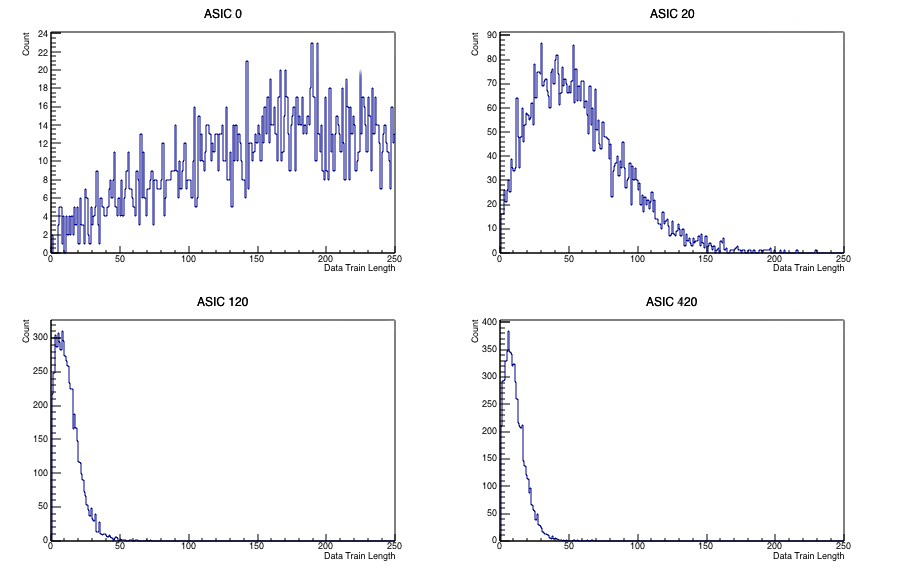
\includegraphics[width=\textwidth]{asic_datatrain_length}
	% 		\caption{The data train length distribution of 4 ASIC chips.}
	% 		\label{fig:asic_datatrain}
	% 	\end{figure}
	% 	\par
	% 	\begin{figure}[h]
	% 		\centering
	% 		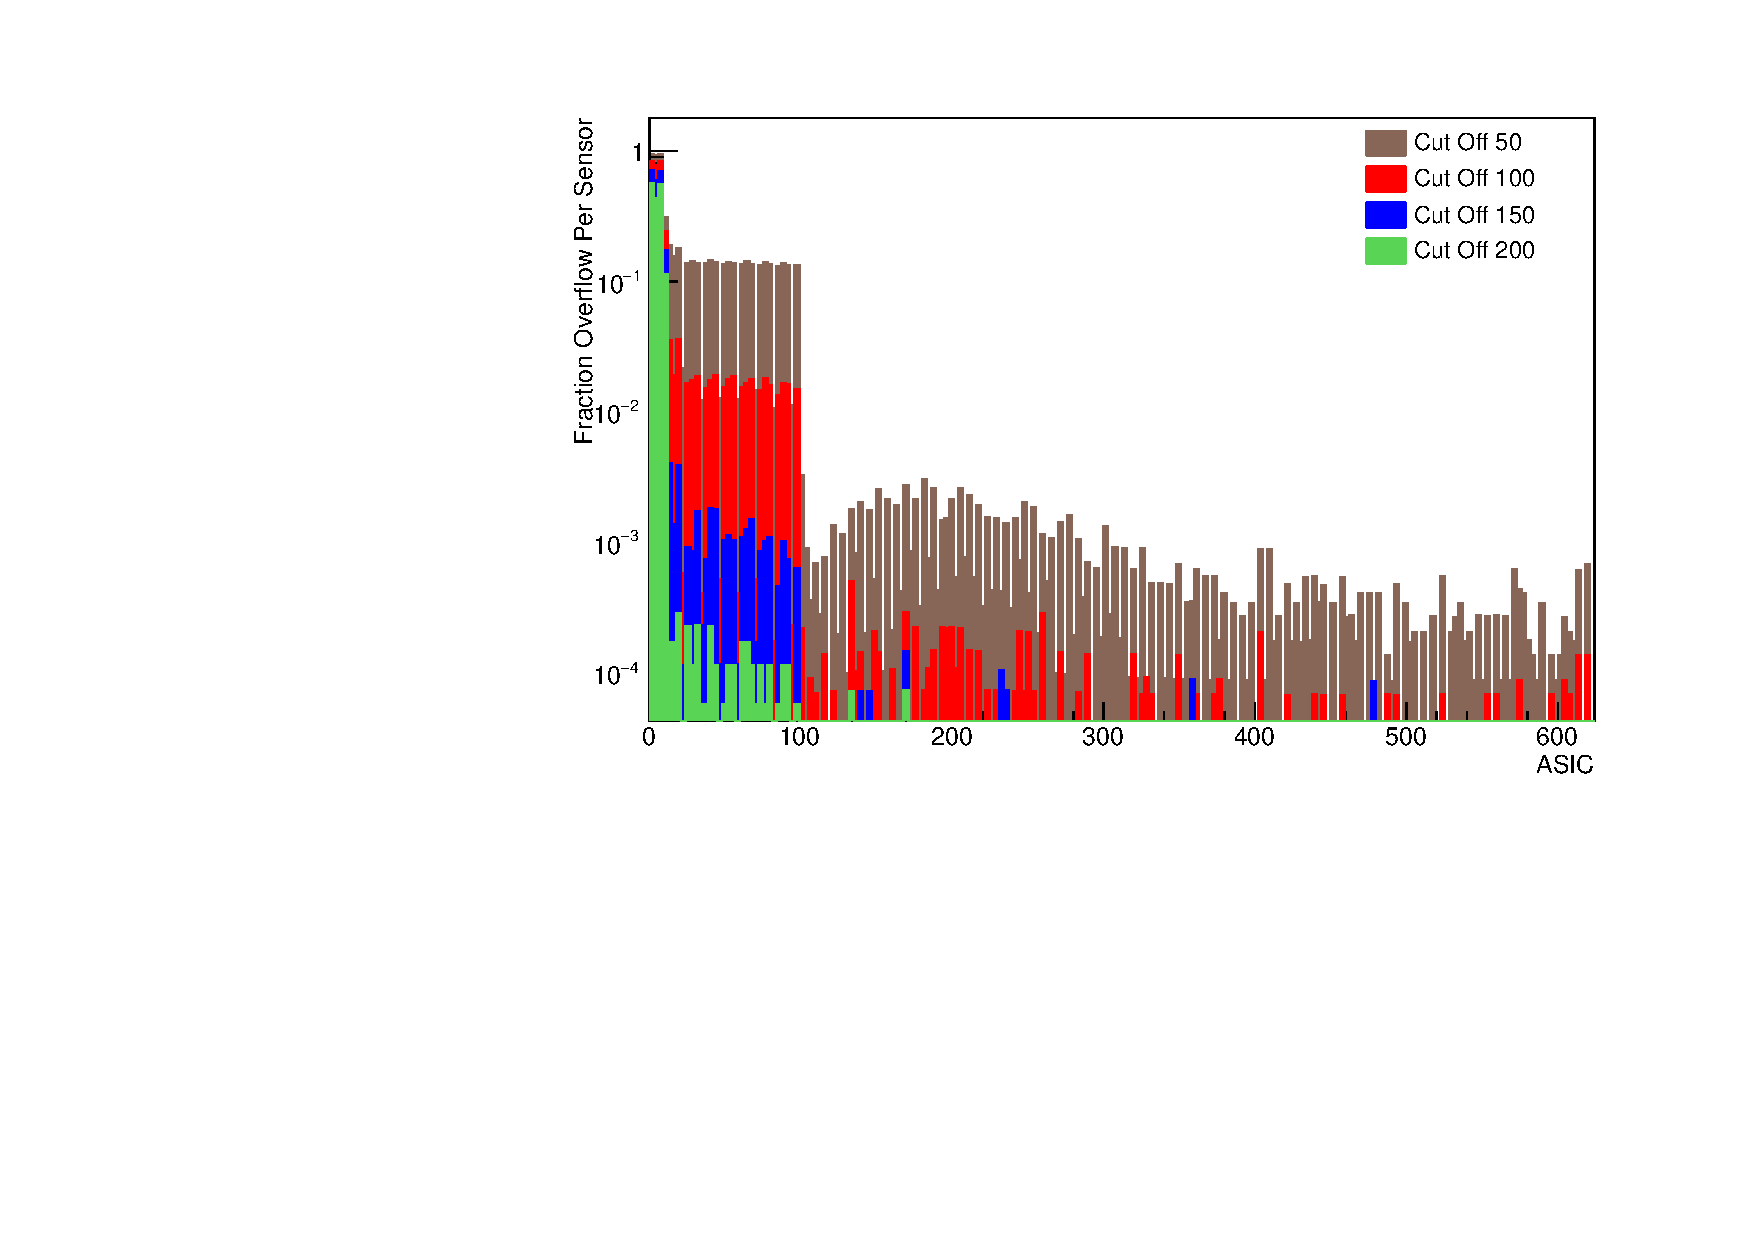
\includegraphics[width=0.7\textwidth]{overflow_graph.pdf}
	% 		\caption{fraction of overflow data trains for four overflow limits.}
	% 		\label{fig:overflow_franction}
	% 	\end{figure}\FloatBarrier
	% 	More important, however, is the fraction of data trains over the bypass limit.
	% 	For four hypothetical limits, the fraction of overflow data trains was calculated from the VELO simulated data, and is shown in Figure~\ref{fig:overflow_franction}.
	% 	This analysis, however, raises questions beyond that of the overflow limit.
	% 	The ASICs below 100 show no simulatity to those above 100.

	% 	\begin{figure}[h]
	% 		\centering
	% 		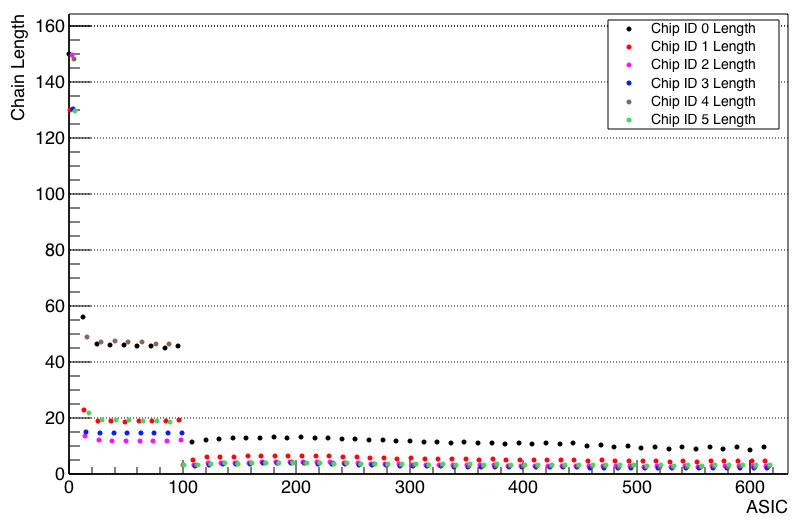
\includegraphics[width=0.49\textwidth]{Mean_ASIC_Graph_Chip}
	% 		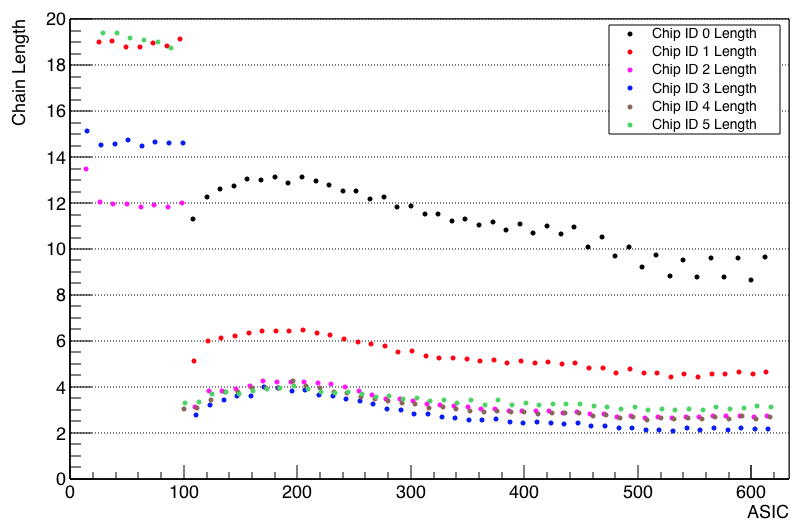
\includegraphics[width=0.49\textwidth]{Mean_ASIC_Graph_Chip_lower_values}
	% 		\caption{The mean data train length for each ASIC, coloured by the chip number.}
	% 		\label{fig:asic_structure}
	% 	\end{figure}\FloatBarrier
	% 	Further investigations as to the structure of the simulated data is shown in Figure~\ref{fig:asic_structure}.
	% 	Here the data is partitioned by the position of the ASIC chip in the module.
	% 	From this we learn that large variance in the data (ASIC number $>$ 100) is due to the ASICs position on the module.
	% 	This result is expected as the ASICs closer to the beam line will detect more particle paths.
	% 	However, this structure is not consistaent across the ASIC's pre and post 100.
	% 	It can be concuded that the simulated data contains a \textit{`bug'}.
	% 	This \textit{`bug'} is now being reviewed by the creators of the simulation. 
	% 	No further analysis can be continued on setting an overflow limit until this \textit{`bug'} has been properly investigated.

	% 	% subsection data_train_overflowa (end)

	% \subsection{Current Stage of Development} 
	% 	The EIF system is still currently in active VHDL development.
	% 	The current developmental code is still in a stand alone format and not intergrated with the master LLI code.
	% 	Currently created and ready for stand alone testing, is a bubble sorting module with data in and out systems.
	% 	The module consists of a top level control entity and a comparison/swap sorting entity.
	% 	The control entity forms a feedback loop passing the ouput of the sorting enity back into its input at each step.
	% 	At each step, the parity of comparison is changed (i.e. odd-even to even-odd).
	% 	\begin{figure}[h]
	% 		\centering
	% 		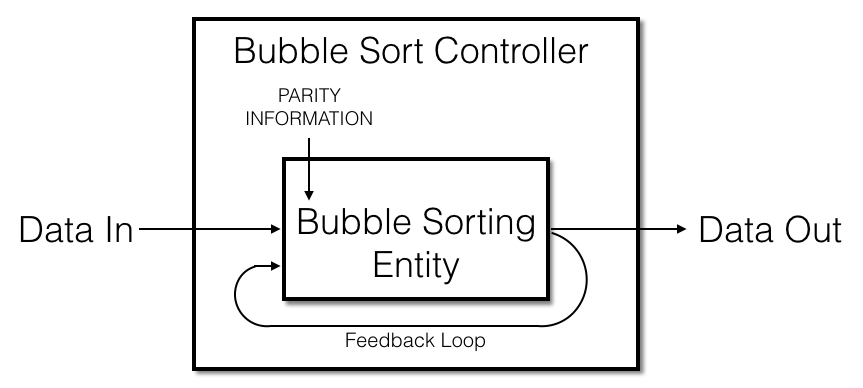
\includegraphics[width=0.65\textwidth]{bubblesort_modual}
	% 		\caption{Data from for the developmental bubble sorting module.}
	% 		\label{fig:bubble_data_flow}
	% 	\end{figure} \FloatBarrier
	% 	\par
	% 	This process continues until the input and output of the sorting module is identical for two subsequent steps.
	% 	At this point the data is sorted and passed to the output.
	% 	The data flow is more simply demonstrated in Figure~\ref{fig:bubble_data_flow}.
	% 	\par
	% 	Once testing of the bubble sorting is complete and the simulated data bug is fixed, the EIF will be expanded to include Isolation Flagging and an overflow, as discussed.
	% 	Once the stand alone system is complete, it will be intergrated into the LLI master code and modified to comply with the LLI data management systems.
		\FloatBarrier